\documentclass[12pt]{article}

\usepackage{listings}
\lstset{
  language=Haskell
}

\usepackage{graphicx}
\graphicspath{ {../resources/what-is-the-web/} }

\usepackage[margin=1in]{geometry}

\usepackage[colorlinks]{hyperref}
\hypersetup{
  urlcolor = {cyan}
}

\newcommand{\tightlist}{\setlength{\itemsep}{0pt}\setlength{\parskip}{0pt}}

\title{What is the Web}
\author{Rushi Shah}
\date{18 February 2016}

\begin{document}

  \maketitle

  %https://www.w3.org/People/Raggett/book4/ch02.html

  You use the internet, like every day, right? But at its core, what is the web? I don't think it is really anything more than a web of interconnected documents that link to each other. You can explore this massive graph of HTML pages to find what you want to see. Here is a figure that represents a simplified view of the internet as a series of documents. 

  %Image of interconnected documents
  \begin{center}
  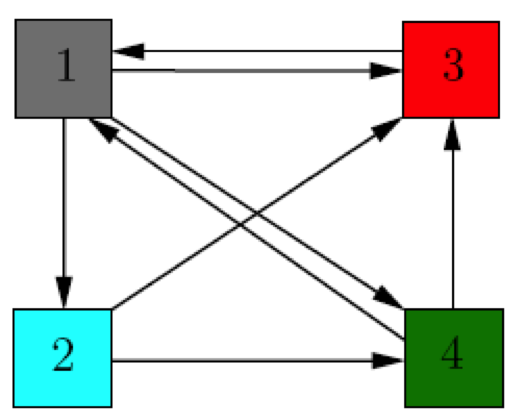
\includegraphics[height=3in]{documents}
  \end{center}

  Seems simple enough, right? This graphic was actually used in a presentation I saw about how Google's Page Rank algorithm works, but I thought it was an appropriate depiction of what the internet really is for our purposes. My (perhaps slightly rhetorical) question is, why are we so chained to a web of only HTML files?

  \section{HTML}

  To be clear, I have no quarrell with HTML. It is impressive how standardized it is, especially considering the tech-community's bad habit of splintering standards (I'm looking at every one of you 7 billion JS frameworks!). And because it is so standard, browswers don't need to worry about supporting the latest and ``greatest'' file format.

  \section{PDFs}

  But I think PDFs are more than just a file fad. So much so that every major browswer (Chrome, Safari, Firefox) has built in support for viewing PDFs in the browser. So imagine for a moment that every page on the web was just a PDF rather than an HTML page. Not much would fundamentally change, because both PDFs and HTML have the same funcionality. 

  Theoretically exactly nothing would change. You can style PDFs just like you can use CSS. Techincally LaTeX is Turing complete so everything you can do with Javascript can be done in PDFs. But I'm not talking about grandiose and unrealistic claims. I'm just saying that PDFs aren't all that different from HTML, especially because we only use a small portion of HTML's already limited functionality. 

  \section{Blogs}

  Take your standard tech-blog, for example. What does it need? It needs a set of interconnected documents that you can access from one another and read. It needs links to other documents in case you want further information. It needs to look nice (arguably). It needs to be able to display pictures and figures. It needs some basic formatting capabilities (bold, italic, headers, lists, etc.). 

  PDFs can do all of those things without stretching their capabilities! The only thing is that we are so used to HTML that we don't break out of the status quo. But there is no reason that we can't, right? 

  \section{Why lol?}

  Okay so hypothetically you \textit{could} replace HTML documents with PDF documents. But why, you may ask. I had a couple of reasons for creating BlaTeX, some more valid than others. 

  \subsection{LaTeX \textgreater  Markdown}

  This is probably one of the most arguable points. So let me start off by saying \textbf{This is all a matter of personal preference!} The entire next section is just my opinion. 

  With that out of the way, let me get down to it. I am not personally a big fan of Markdown. I get that its easy to use, but it doesn't feel very expressive to me. I prefer LaTeX. I think LaTeX is fun to write in. But LaTeX doesn't compile to HTML. It compiles to PDF. That's actually how this whole thing started. One day, I was writing a blog post and I wanted to embed the Rayleigh equation 

  \begin{displaymath}
  I \propto \frac{1}{\lambda^4}
  \end{displaymath}

  and my cursory google search was not fruitful. I didn't find any simple and sustainable solution for embedding a simple equation like this into Markdown. After telling this story a few times, people have pointed out a few decent solutions to me, but that's besides the point. The point is that LaTeX is the best tool for the job. I just want to write my blog posts in LaTeX! And let's be honest, the kind of crowd that my blog would attract (which is admittedly a rather miniscule crowd to begin with) would sympathize with me. I hope they wouldn't blame me for wanting to use LaTeX. 

  \subsection{These are some of my favorite things}  

  PDFs are underrated. LaTeX is solid. And blogging is a party. So like gluing all three together with a bit of Haskell is the dream, right?

  \begin{center}
  
\includegraphics[height=2in]{favorite_things}
  \end{center}


  \subsection{It's kind of neat.}

  Why do I like PDFs so much? I don't know, I just think they're kind of neat. 
  % http://s2.quickmeme.com/img/b4/b48c976ada123eeec32d3063af01f9915a659ac554897314d8fd54ff8939788f.jpg
  \begin{center}
  
\includegraphics[height=2in]{neat}
  \end{center}

  \subsection{For Science!}

  Full disclosure, BlaTeX was my senior research project at Thomas Jefferson High School for Science and Technology. So in reality, I made this for science. It was like an experiment: ``Hey, what would happen if instead of HTML pages, you just used PDFs yo!''. But aren't those types of things the best projects?

  % include image of the for science guy

  \subsection{Why not?}

  I feel like an unwritten rule nowadays is that if it can be done, it will be done. So like don't ask me why I wanted to replace HTML pages with PDF pages, ask yourself why it wasn't done sooner. 

  \section{TL;DR}

  The web is just a series of interconnected documents, and I don't see any reason they can't be PDF documents (especially because by switching, blog authors can use LaTeX). 

\end{document}